\section{Black-Scholes Model}
\label{sect:bs-model}
\begin{enumerate}
\item The binomial option pricing model, regardless of how many periods it has,
is still inherently \emph{discrete}: There are finitely many distinct terminal
stock prices and finitely many time points involved.

\item The most famous model in the \emph{continuous} realm (where a ``stream''
of distinct terminal stock prices and time points is involved) is perhaps the
\emph{Black-Scholes model} --- the model we study here.
\end{enumerate}
\subsection{Model Formulation}
\begin{enumerate}
\item Before specifying the Black-Scholes model, we first discuss a closely
related concept: \emph{lognormal distribution}.

\item A random variable \(Y\) follows a \defn{lognormal distribution} with
parameters \(\mu\) and \(\sigma^2\) (denoted by \(Y\sim
\text{\(LN(\mu,\sigma^2)\)}\)) if the ``log'' of \(Y\), \(\ln Y\),
follows a normal distribution with mean \(\mu\) and variance \(\sigma^2\),
i.e., \(\ln Y\sim N(\mu,\sigma^2)\).

\begin{warning}
The parameters \(\mu\) and \(\sigma^2\) are \emph{not} the mean and variance of
\(Y\)!
\end{warning}

\item \label{it:ln-dist-mean-var}
To compute moments of \(Y\), it is useful to recall that the moment
generating function of a normal r.v. \(X\sim N(\mu,\sigma^2)\):
\[
M_X(t)=\expv{e^{tX}}=\exp\qty(\mu t+\frac{1}{2}\sigma^2t^2).
\]
Since \(Y=e^{X}\), the first and second moments of \(Y\) are
\[
\expv{Y}=\expv{e^X}=M_X(1)=e^{\mu+\sigma^2/2},
\]
and
\[
\expv{Y^2}=\expv{e^{2X}}=M_X(2)=e^{2(\mu+\sigma^2)}.
\]
Hence, the variance of \(Y\) is
\[
\vari{Y}=\expv{Y^2}-\qty(\expv{Y})^{2}=e^{2\mu+\sigma^2}\qty(e^{\sigma^2}-1).
\]

\item \label{it:bs-model-def}
In the \defn{Black-Scholes model} (or \defn{Black-Scholes framework}), we are
assumed to be in a perfect market having the following two assets:
\begin{itemize}
\item a risky stock \faIcon{apple-alt} which pays dividend continuously
at a dividend yield \(\delta\), where its time-\(t\) price is
\[
S_t=S_0\exp\qty[\qty(\alpha-\delta-\frac{\sigma^2}{2})t+\sigma\sqrt{t}Z_t],
\]
for some nonnegative parameters \(\alpha\) and \(\sigma\), and some
\emph{standard normal} random variable \(Z_t\)'s that are ``related in a
certain way'';
\item a (risk-free zero-coupon) bond \faIcon{file-invoice-dollar} with an
annual continuously compounded risk-free rate \(r\).
\end{itemize}

\begin{remark}
\item A more technical and precise definition (discussed in STAT3911) of the
Black-Scholes model involves the notion of \emph{geometric Brownian motion}
(that describes how the \(Z_t\)'s are ``related''), which we shall omit here.

\item As we can see, the Black-Scholes model is like a ``continuous analogue''
to binomial option pricing model (the setting is ``similar''; just that the
stock price evolves \emph{continuously} rather than in a discrete manner).
Indeed, it turns out that the Black-Scholes model can be obtained as a
\emph{limit} of multi-period binomial option pricing model (no.\ of periods
\faIcon{arrow-up} \& duration of each period \faIcon{arrow-down}).

\item Although the expression for \(S_t\) appears to be complex and not so
intuitive, it makes the parameters \(\alpha\) and \(\sigma\) more easily
interpretable. (See \labelcref{it:alpha-sigma-interpret}.)
\end{remark}

\item The Black-Scholes model is related to the concept of lognormal
distribution, since we have
\[
\ln S_t=\ln S_0+\qty(\alpha-\delta-\frac{\sigma^2}{2})t+\sigma\sqrt{t}Z_t,
\]
where \(Z_t\sim N(0,1)\), which implies
\[
\ln S_t\sim N\qty[\ln S_0+\qty(\alpha-\delta-\frac{\sigma^2}{2})t,\sigma^2t],
\]
or
\[
S_t\sim LN\qty[\ln S_0+\qty(\alpha-\delta-\frac{1}{2}\sigma^2)t,\sigma^2t].
\]
\item \label{it:bs-model-return-normal}
In the Black-Scholes model, the \(t\)-year continuously compounded rate of
\emph{price} return on the stock \faIcon{apple-alt} (i.e., continuous dividend
is not considered in the calculation of return) is
\[
\ln\frac{S_t}{S_0}=\qty(\alpha-\delta-\frac{\sigma^2}{2})t+\sigma\sqrt{t}Z_t
\sim N\qty[\qty(\alpha-\delta-\frac{\sigma^2}{2})t,\sigma^2t].
\]
So, in the Black-Scholes model, while \emph{stock prices} are lognormally
distributed, the \emph{continuously compounded returns} are normally
distributed.

\item \label{it:alpha-sigma-interpret}
Interpretations of \(\alpha\) and \(\sigma\):
\begin{itemize}
\item \(\alpha\): By the mean formula in \labelcref{it:ln-dist-mean-var},
\[
\expv{S_t}=\exp\qty[\ln S_0+\qty(\alpha-\delta-\frac{\sigma^2}{2})t+\frac{\sigma^2}{2}t]
=S_0e^{(\alpha-\delta)t},
\]
which means
\[
e^{\alpha t}-1=\expv{\frac{e^{\delta t}S_t-S_0}{S_0}}.
\]
Since \((e^{\delta t}S_t-S_0)/S_0\) is the \(t\)-year rate of total return
on the stock \faIcon{apple-alt}\footnote{To be more precise, it is the rate of
return on a \emph{portfolio} containing a share of stock. Both the
\faIcon{arrow-up} in no.\ of shares owned from continuous dividend and the
\faIcon{arrow-up} in stock price contribute to the \faIcon{arrow-up} in
\emph{portfolio} value.}, it follows that \(\alpha\) is the continuously
compounded expected rate of return on the stock \faIcon{apple-alt} (or ``log
expected return'').
\begin{remark}
\item Although \(\alpha\) should be interpreted as ``log expected return'',
sometimes it is (improperly) called ``expected log return''.  \item It turns
out that for \emph{option pricing purpose}, the value of \(\alpha\) does not
matter. (See \cref{sect:bs-pricing-fmla}.) This is analogous to the property
that the \emph{true} probability \(p\) does not affect the option pricing in
binomial option pricing model.
\end{remark}
\item \(\sigma\): By \labelcref{it:bs-model-return-normal},
\[
\vari{\ln\frac{S_t}{S_0}}=\sigma^2t
\implies
\sigma=\sqrt{\frac{1}{t}\vari{\ln\frac{S_t}{S_0}}}.
\]
Hence, \(\sigma\) is the volatility of the stock \faIcon{apple-alt} (hence the
notation \(\sigma\)).
\end{itemize}
\begin{figure}[!h]
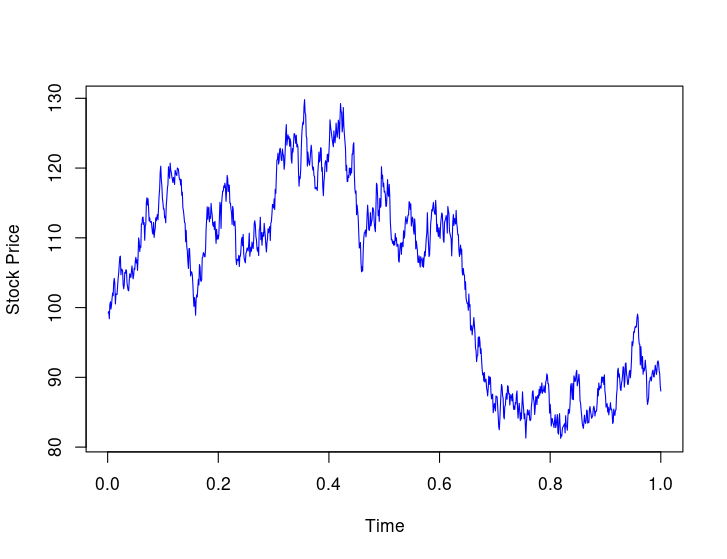
\includegraphics{images/bs-stock-price}
\caption{A simulated stock price path under the Black-Scholes model with
\(S_0=100\), \(\alpha=0.12\), \(\delta=0.02\), and \(\sigma=0.4\).}
\begin{minted}[bgcolor=gray!10!white]{R}
#R code
set.seed(1)
N <- 1000
S0 <- 100
alpha <- 0.12
delta <- 0.02
sigma <- 0.4

time_pts <- (1:N)/N
dt <- 1/N
Wt <- cumsum(rnorm(N)) * sqrt(dt)
St <- S0 * exp((alpha - delta - sigma^2/ 2) * time_pts + sigma * Wt)
plot(time_pts, St, col="blue", type="l", xlab="Time", ylab="Stock Price")
\end{minted}
\end{figure}
\end{enumerate}
\subsection{Probabilistic Quantities Under Black-Scholes Model}
\begin{enumerate}
\item Although the main usage of Black-Scholes model is option pricing, we can
indeed compute some probabilistic quantities concerning the \emph{stock}
\faIcon{apple-alt} of theoretical/practical interest, based on the
specification of its stock price in the Black-Scholes model.
\subsubsection*{Exercise Probabilities}
\item The first quantity is also related to option: the (true) probability that
an European call on the stock \faIcon{apple-alt} will be exercised (by a
rational holder) at expiration (the \defn{exercise probability} of the call),
i.e.,
\(\prob{S_T>K}\).
\item \label{it:bs-exercise-prob-fmla}
The probability is given by:
\begin{align*}
\prob{S_T>K}&=\prob{\ln S_T>\ln K}\\
&=\prob{\ln S_0+\qty(\alpha-\delta-\frac{\sigma^2}{2})T+\sigma\sqrt{T}Z_T>\ln K}\\
&=\prob{Z_T>\frac{\ln(K/S_0)-(\alpha-\delta-\sigma^2/2)T}{\sigma\sqrt{T}}}\\
&=\prob{{\color{Maroon}-}Z_T<{\color{violet}\frac{\ln(S_0/K)+(\alpha-\delta-\sigma^2/2)T}{\sigma\sqrt{T}}}}\\
&=\Phi({\color{violet}\widehat{d_2}})&(-Z_T\sim N(0,1)\text{ also})
\end{align*}
where \(\Phi(\cdot)\) is the standard normal cdf, and 
\[
\text{\(\widehat{d_2}\)}=\frac{\ln(S_0/K)+(\alpha-\delta-\sigma^2/2)T}{\sigma\sqrt{T}}.
\]
\begin{note}
We shall discuss why the notation ``\(\widehat{d_2}\)'' is used here in
\cref{sect:bs-pricing-fmla}.
\end{note}
\item Then, the exercise probability of an otherwise identical European
\emph{put} is
\[
\prob{S_T<K}=1-\prob{S_T>K}=1-\Phi(\widehat{d_2})=\Phi(-\widehat{d_2}).
\]
\subsubsection*{Lognormal Prediction Intervals for Stock Prices}
\item The next quantity of interest is a range of values in which the stock
price has a high probability of lying (useful for ``predicting'' future stock
price!).
\item For any \(t\ge 0\) and \(p\in (0,1)\) ``close to'' 0 (so that the
probability of lying is ``high''), we want to find (nonrandom) constants
\(S^L\) and \(S^U\) such that
\[
\prob{S^L<S_t<S^U}=1-p.
\]
The interval \([S^L,S^U]\) is called a \defn{\(100(1-p)\)\% lognormal
prediction interval} for \(S_t\).

\begin{remark}
\item Often we want to find an \defn{equal-tailed} lognormal prediction
interval, i.e.,
\[
\prob{S_t<S^L}=\prob{S_t>S^U}=\frac{p}{2}.
\]
\item You may have learnt about the concept of \emph{confidence interval} in
your statistics course and find this concept to be ``similar''. The differences
between the concepts of \emph{confidence intervals} and \emph{prediction
intervals} are given below:

\begin{center}
\begin{tabular}{ccc}
\toprule
Type&Bounds of intervals are:&Target is:\\
\midrule
confidence interval&random variables&(nonrandom) constant\\
prediction interval&(nonrandom) constants&random variable\\
\bottomrule
\end{tabular}
\end{center}
\end{remark}
\item \label{it:bs-equal-tailed-ln-pi}
To find a \(100(1-p)\%\) prediction interval for \(S_t\) for any \(t\ge
0\), we start with the equation
\[
\prob{\Phi^{-1}\qty(\frac{p}{2})<Z_t<\Phi^{-1}\qty(1-\frac{p}{2})}=1-p.
\] \begin{center}
\begin{tikzpicture}
\begin{axis}[
domain=-3:3,
samples=75,
axis lines=center,
xmin=-3.5,xmax=3.5,
ymax=0.5,
xtick={-2,2}, xticklabels={\(\Phi^{-1}\qty(\frac{p}{2})\), \(\Phi^{-1}\qty(1-\frac{p}{2})\)},
ytick=\empty,
title={\color{blue}Standard normal pdf \(\phi\)}
]
\addplot[blue, thick, name path=A]{(1/sqrt(2*pi))*exp(-x^2/2)};
\addplot[draw=none, name path=B]{0};
\addplot[violet, opacity=0.3] fill between[of=A and B, soft clip={domain=-2:2}];
\addplot[ForestGreen!50!white] fill between[of=A and B, soft clip={domain=-3:-2}];
\addplot[ForestGreen!50!white] fill between[of=A and B, soft clip={domain=2:3}];
\node[blue] () at (2,0.3) {\(\phi\)};
\node[] () at (0,0.1) {area = \(1-p\)};
\draw[-Latex] (-2.7,0.1) -- (-2.5,0.01)
node[pos=-0.3]{\(p/2\)};
\draw[-Latex] (2.7,0.1) -- (2.5,0.01)
node[pos=-0.3]{\(p/2\)};
\end{axis}
\end{tikzpicture}
\end{center}
After that, since
\[
S_t={\color{violet}S_0\exp\qty[\qty(\alpha-\delta-\frac{\sigma^2}{2})t+\sigma\sqrt{t}{\color{teal}Z_t}]},
\]
we readily have
\[
\prob{
{\color{violet}S_0e^{\qty(\alpha-\delta-\frac{\sigma^2}{2})t+\sigma\sqrt{t}{\color{teal}\Phi^{-1}(p/2)}}}
<S_t<
{\color{violet}S_0e^{\qty(\alpha-\delta-\frac{\sigma^2}{2})t+\sigma\sqrt{t}{\color{teal}\Phi^{-1}(1-p/2)}}}
}=1-p.
\]
It follows that the \(100(1-p)\)\% \emph{equal-tailed} prediction interval for
\(S_t\) is
\[
\qty[
S_0\exp\qty{\qty(\alpha-\delta-\frac{\sigma^2}{2})t+\sigma\sqrt{t}\Phi^{-1}\qty(\frac{p}{2})},
S_0\exp\qty{\qty(\alpha-\delta-\frac{\sigma^2}{2})t+\sigma\sqrt{t}\Phi^{-1}\qty(1-\frac{p}{2})}
].
\]
\item The following are some non-equal-tailed \(100(1-p)\)\% prediction
intervals:
\begin{itemize}
\item \(\displaystyle \left(0,S_0\exp\qty{\qty(\alpha-\delta-\frac{\sigma^2}{2})t+\sigma\sqrt{t}\Phi^{-1}(1-p)}\right]\)
\item \(\displaystyle \qty(S_0\exp\qty{\qty(\alpha-\delta-\frac{\sigma^2}{2})t+\sigma\sqrt{t}\Phi^{-1}(p)},\infty)\)
\end{itemize}
\begin{pf}
Start with the equations
\[
\prob{-\infty<Z_t<\Phi^{-1}(1-p)}=1-p,
\]
and
\[
\prob{\Phi^{-1}(p)<Z_t<\infty}=1-p
\]
respectively, and note that \(e^{x}\to \infty\) (\(0\)) as \(x\to
\infty\) (\(-\infty\)).
\end{pf}

These prediction intervals are sometimes called \defn{one-sided} or
\defn{one-tailed}.
\subsubsection*{Conditional Expected Stock Prices}
\item \label{it:bs-exp-stock-price}
This quantity is again somewhat related to option also. We know that the
(unconditional) expected time-\(t\) stock price is
\(\expv{S_t}=S_0e^{(\alpha-\delta)t}\) by \labelcref{it:alpha-sigma-interpret}.

\item Given an European call (put) expiring at time \(T\), we are sometimes
interested in knowing the expected \emph{terminal} (i.e., time-\(T\)) stock
price, given the call (put) expires \emph{in-the-money}, i.e., \(S_T>K\)
(\(K>S_T\)) \faIcon{arrow-right} gets exercised.\footnote{Intuitively, this
conditional expected value can measure the ``extent'' of the gain (loss) for
the option holder (writer) on average when the option gets exercised.} So we
want to find the conditional expectation \(\expv{S_T|S_T>K}\)
(\(\expv{S_T|S_T<K}\)).

\item The following gives the formula for \(\expv{S_T|S_T>K}\) and
\(\expv{S_T|S_T<K}\):
\begin{proposition}
\label{prp:bs-exp-stock-price-given-itm}
Under the Black-Scholes model, we have
\[
\expv{S_T|S_T>K}=S_0e^{(\alpha-\delta)T}\frac{\Phi(\widehat{d_1})}{\Phi(\widehat{d_2})}
\]
and
\[
\expv{S_T|S_T<K}=S_0e^{(\alpha-\delta)T}\frac{\Phi(-\widehat{d_1})}{\Phi(-\widehat{d_2})}
\]
where \(\displaystyle
\widehat{d_2}=\frac{\ln(S_0/K)+(\alpha-\delta-\sigma^2/2)T}{\sigma\sqrt{T}}\)
(recall) and \(\text{\(\widehat{d_1}\)}=\widehat{d_2}+\sigma\sqrt{T}.\)
\end{proposition}
\begin{intuition}
Both expressions are of the form \[\text{unconditional expected stock
price}\times\text{adjustment factor}.\]
\begin{itemize}
\item For \(\expv{S_T|S_T>K}\), the adjustment factor is
\(\Phi(\widehat{d_1})/\Phi(\widehat{d_2})>1\) (as \(\widehat{d_1}>\widehat{d_2}\));
\item For \(\expv{S_T|S_T<K}\), the adjustment factor is
\(\Phi(-\widehat{d_1})/\Phi(-\widehat{d_2})<1\) (as \(-\widehat{d_1}< -\widehat{d_2}\)).
\end{itemize}
So, intuitively, conditioning on \(S_T>K\) (\(S_T\) is ``of high
value'')/\(S_T<K\) (\(S_T\) is ``of low value'') increases/decreases the
expected value.
\end{intuition}

\begin{pf}
Consider first \(\expv{S_T|S_T>K}\). Here we use the following formula for
conditional expectation:
\[
\expv{S_T|S_T>K}=\frac{\expv{S_T\indicset{S_T>K}}}{\prob{S_T>K}}.
\]
(By \labelcref{it:bs-exercise-prob-fmla}, we have \(\prob{S_T>K}=\prob{Z_T>
-\widehat{d_2}}=\Phi(\widehat{d_2})>0\).)
Now, we compute
\begin{align*}
\expv{S_T\indicset{S_T>K}}&=\expv{S_0\exp\qty{\qty(\alpha-\delta-\frac{\sigma^2}{2})T+\sigma\sqrt{T}Z_T}\indicset{Z_T> -\widehat{d_2}}} \\
&=\int_{-\infty}^{\infty}S_0\exp\qty{\qty(\alpha-\delta-\frac{\sigma^2}{2})T+\sigma\sqrt{T}{\color{violet}z}}\indicset{{\color{violet}z}> -\widehat{d_2}}\phi({\color{violet}z})\,dz\\
&=S_0e^{(\alpha-\delta)T}\int_{-\widehat{d_2}}^{\infty}e^{\color{teal}-(\sigma^2/2)T+\sigma\sqrt{T}z}\frac{1}{\sqrt{2\pi}}e^{\color{teal}-z^2/2}\,dz\\
&=S_0e^{(\alpha-\delta)T}\int_{-\widehat{d_2}}^{\infty}\frac{1}{\sqrt{2\pi}}e^{\color{teal}-(z-\sigma\sqrt{T})^{2}/2}\,dz\\
&=S_0e^{(\alpha-\delta)T}\int_{-\widehat{d_2}-\sigma\sqrt{T}}^{\infty}\frac{1}{\sqrt{2\pi}}e^{\color{teal}-u^2/2}\,du&(u=z-\sigma\sqrt{T})\\
&=S_0e^{(\alpha-\delta)T}(\underbrace{1-\Phi(-\widehat{d_1})}_{\Phi(\widehat{d_1})})
\end{align*}
where \(\phi(\cdot)\) is the standard normal pdf.
\begin{center}
\begin{tikzpicture}
\begin{axis}[
domain=-3:3,
samples=75,
axis lines=center,
xmin=-3.5,xmax=3.5,
ymax=0.5,
xtick={-2,2}, xticklabels={\(-\widehat{d_1}\), \(\widehat{d_1}\)},
ytick=\empty,
]
\addplot[blue, thick, name path=A]{(1/sqrt(2*pi))*exp(-x^2/2)};
\addplot[draw=none, name path=B]{0};
\addplot[violet, opacity=0.3] fill between[of=A and B, soft clip={domain=-2:3}];
\addplot[ForestGreen!50!white] fill between[of=A and B, soft clip={domain=-3:-2}];
\node[blue] () at (2,0.3) {\(\phi\)};
\draw[-Latex] (-2.7,0.1) -- (-2.5,0.01)
node[pos=-0.3]{\(\Phi(-\widehat{d_1})\)};
\draw[-Latex] (2,0.2) -- (1,0.1)
node[pos=-0.3]{\(1-\Phi(-\widehat{d_1})\)};
\end{axis}
\end{tikzpicture}
\begin{tikzpicture}
\begin{axis}[
domain=-3:3,
samples=75,
axis lines=center,
xmin=-3.5,xmax=3.5,
ymax=0.5,
xtick={-2,2}, xticklabels={\(-\widehat{d_1}\), \(\widehat{d_1}\)},
ytick=\empty,
]
\addplot[blue, thick, name path=A]{(1/sqrt(2*pi))*exp(-x^2/2)};
\addplot[draw=none, name path=B]{0};
\addplot[ForestGreen!50!white] fill between[of=A and B, soft clip={domain=2:3}];
\addplot[violet, opacity=0.3] fill between[of=A and B, soft clip={domain=-3:2}];
\node[blue] () at (2,0.3) {\(\phi\)};
\draw[-Latex] (-2,0.2) -- (-1,0.1)
node[pos=-0.3]{\(\Phi(\widehat{d_1})\)};
\draw[-Latex] (2.7,0.1) -- (2.5,0.01)
node[pos=-0.3]{\(1-\Phi(\widehat{d_1})\)};
\end{axis}
\end{tikzpicture}
\end{center}
It then follows that 
\[
\expv{S_T|S_T>K}=S_0e^{(\alpha-\delta)T}\frac{\Phi(\widehat{d_1})}{\Phi(\widehat{d_2})}.
\]
Now, for \(\expv{S_T|S_T<K}\), apply law of total expectation gives
\[
\expv{S_T}=\expv{S_T|S_T>K}\prob{S_T>K}+\expv{S_T|S_T<K}\prob{S_T<K},
\]
which implies
\[
S_0e^{(\alpha-\delta)T}=S_0e^{(\alpha-\delta)T}\Phi(\widehat{d_1})
+\expv{S_T|S_T<K}\Phi(-\widehat{d_2}),
\]
and thus
\[
\expv{S_T|S_T<K}=S_0e^{(\alpha-\delta)T}\frac{\Phi(-\widehat{d_1})}{\Phi(-\widehat{d_2})}.
\]
(Note that \(1-\Phi(\widehat{d_1})=\Phi(-\widehat{d_1})\).)
\end{pf}
\end{enumerate}
